\section{Übertragungsfunktionen der gemessenen Daten}
Aus den Messkurven geht hervor, dass der Prozess ein PT$_1$-Glied darstellt
in beiden Arbeitspunkten. Die Übertragungsfunktionen zu den Arbeitspunkteen
ist aus den Sprungantworten hergeleitet nach dem Zeit-Prozent-Verfahren. Da
der Prozess zu zwei Arbeitspunkten betrachtet wird, sollen die folgenden
Konventionen gelten:

\begin{table}[h!]
	\centering
	\begin{tabular}{l l}
		Bezeichner & Bedeutung \\
		\hline
		$\tau_5$ & Zeitkonstante im Arbeitspunkt 5V \\
		$K_{g_5}$ & Proportionalkonstante im Arbeitspunkt 5V \\
		$\tau_7$ & Zeitkonstante im Arbeitspunkt 7V \\
		$K_{g_7}$ & Proportionalkonstante im Arbeitspunkt 7V 
	\end{tabular}
\end{table}

\subsection{Sprungantwort von 5V zu 5.5V}
Aus den Messdaten gehen die folgenden Werte hervor
\begin{table}[h!]
	\centering
	\begin{tabular}{l l r}
		Grösse & Bezeichner & Wert \\
		\hline
		Starthöhe & $h_0$ & 2.1\si{\centi\meter} \\
		Endhöhe & $h_\infty$ & 4.5\si{\centi\meter} \\
	\end{tabular}
\end{table}

\subsubsection{Schätzung der Zeitkonstante $\tau_5$}
Aus den obigen Werten ist für die Höhe nach einem $\tau$ ein Wert berechnet
von 
\[
	(h_\infty - h_0) \cdot 63\% + h_0
	= h_{\tau}
	= (4.5\si{\centi\meter} - 2.1\si{\centi\meter}) \cdot 0.63
		+ 2.1\si{\centi\meter}
	= 3.757\si{\centi\meter}
\]
Aus der Messkurve geht hervor, dass diese Höhe nach einer Zeit von ca. 70s
erreicht wird. Diese Zeit entspricht gerade der Zeitkonstante $\tau$ des
Systems. Um dies zu kontrollieren ist eine Kontrollrechnung durchgeführt,
welche die Zeitspanne bis $t = 2\tau$ betrachtet.
\[
	(h_\infty - h_0) \cdot 86\% + h_0
	= h_{2\tau}
	= (4.5\si{\centi\meter} - 2.1\si{\centi\meter}) \cdot 0.86
		+ 2.1\si{\centi\meter}
	= 4.15\si{\centi\meter}
\]
Aus der Messkurve geht hervor, dass diese Höhe nach einer Zeit von ca. 140s
erreicht wird. Da diese Zeit zwei mal der Zeitkonstante $\tau$ entspricht,
ergibt sich wiederum ein $\tau$ von 70s. Der Wert aus der ersten Berechnung
ist somit verifiziert.

\subsubsection{Schätzung des Proportionalkonstante $K_{g_5}$}
Die Proportionalkonstante $K_{g_5}$ entspricht dem Quotienten aus dem
erreichten Höhenunterschied und den eingespielten Steuerunterschied.
\[
	K_{g_5}
	= \frac{\Delta \text{output}}{\Delta \text{input}}
	= \frac{\Delta h}{\Delta q}
	= \frac{h_\infty - h_0}{q_{0^+} - q_{0^-}}
	= \frac{4.5\si{\centi\meter} - 2.1\si{\centi\meter}}{5.5\si{\volt}
		-  5.0\si{\volt}}
	= \frac{2.4\si{\centi\meter}}{0.5\si{\volt}}
	= 4.8 \frac{\si{\centi\meter}}{\si{\volt}}
\]

\subsection{Sprungantwort von 7V zu 8V}
Aus den Messdaten gehen die folgenden Werte hervor
\begin{table}[h!]
	\centering
	\begin{tabular}{l l r}
		Grösse & Bezeichner & Wert \\
		\hline
		Starthöhe & $h_0$ & 11.8\si{\centi\meter} \\
		Endhöhe & $h_\infty$ & 17.6\si{\centi\meter} \\
	\end{tabular}
\end{table}

\subsubsection{Schätzung der Zeitkonstante $\tau_7$}
Aus den obigen Werten ist für die Höhe nach einem $\tau$ ein Wert berechnet
von 
\[
	(h_\infty - h_0) \cdot 63\% + h_0
	= h_{\tau}
	= (17.6\si{\centi\meter} - 11.8\si{\centi\meter}) \cdot 0.63
		+ 11.8\si{\centi\meter}
	= 15.454\si{\centi\meter}
\]
Aus der Messkurve geht hervor, dass diese Höhe nach einer Zeit von ca. 98s
erreicht wird. Diese Zeit entspricht gerade der Zeitkonstante $\tau$ des
Systems. Um dies zu kontrollieren ist eine Kontrollrechnung durchgeführt,
welche die Zeitspanne bis $t = 2\tau$ betrachtet.
\[
	(h_\infty - h_0) \cdot 86\% + h_0
	= h_{2\tau}
	= (17.6\si{\centi\meter} - 11.8\si{\centi\meter}) \cdot 0.86
		+ 11.8\si{\centi\meter}
	= 16.788\si{\centi\meter}
\]
Aus der Messkurve geht hervor, dass diese Höhe nach einer Zeit von ca. 195.8s
erreicht wird. Da diese Zeit zwei mal der Zeitkonstante $\tau$ entspricht,
ergibt sich ein $\tau$ von 97.8s ($\tau_{7_2} - \tau_{7_1}$). Dies ist
sehr nahe am Wert aus der ersten Berechnung und ist somit verifiziert.

\subsubsection{Schätzung des Proportionalkonstante $K_{g_7}$}
Die Proportionalkonstante $K_{g_7}$ entspricht dem Quotienten aus dem
erreichten Höhenunterschied und den eingespielten Steuerunterschied.
\[
	K_{g_7}
	= \frac{\Delta \text{output}}{\Delta \text{input}}
	= \frac{\Delta h}{\Delta q}
	= \frac{h_\infty - h_0}{q_{0^+} - q_{0^-}}
	= \frac{17.6\si{\centi\meter} - 11.8\si{\centi\meter}}{8\si{\volt}
		-  7\si{\volt}}
	= \frac{5.8\si{\centi\meter}}{1\si{\volt}}
	= 5.8 \frac{\si{\centi\meter}}{\si{\volt}}
\]

\subsection{Übertragungsfunktionen \& Modellkontrolle}
Aus den Schätzungen für die Zeit- und Proportionalkonstanten ergeben sich
die folgenden Übertragungsfunktionen.
\[
	G_5(s) 
	= \frac{K_{g_5}}{\tau_5 s + 1} 
	= \frac{4.5\si[per-mode = fraction]{\centi\meter\per\volt}
		}{70\si{\second} \cdot s + 1}
\]
\[
	G_7(s) 
	= \frac{K_{g_5}}{\tau_5 s + 1} 
	= \frac{5.8\si[per-mode = fraction]{\centi\meter\per\volt}
		}{98\si{\second} \cdot s + 1}
\]
Die geschätzten Parameter sind zu einem Modell zusammegefügt und gegen die
Messdaten unter gleichen Bedingungen verglichen.
\begin{figure}[h!]
	\centering
	\begin{subfigure}{0.475\textwidth}
		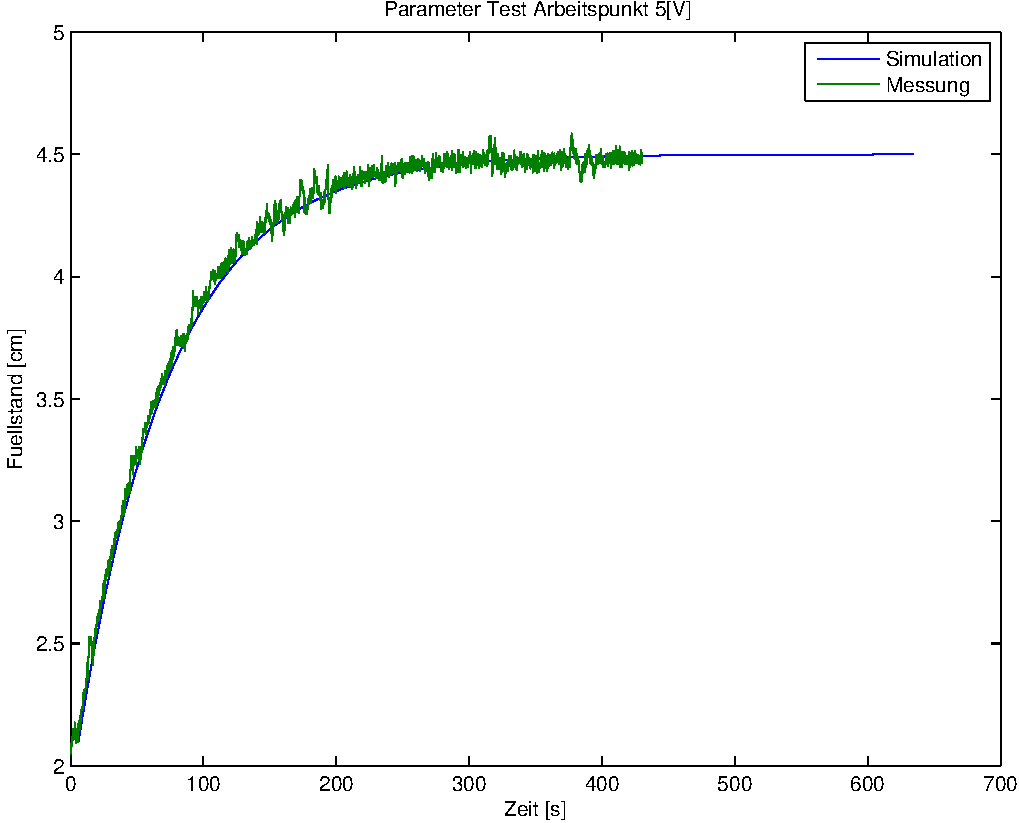
\includegraphics[width=1\textwidth]{07/parameter_test_5.pdf}
		\caption{Sprungantwort 5V zu 5.5V}
	\end{subfigure}
	\hfill{}
	\begin{subfigure}{0.475\textwidth}
		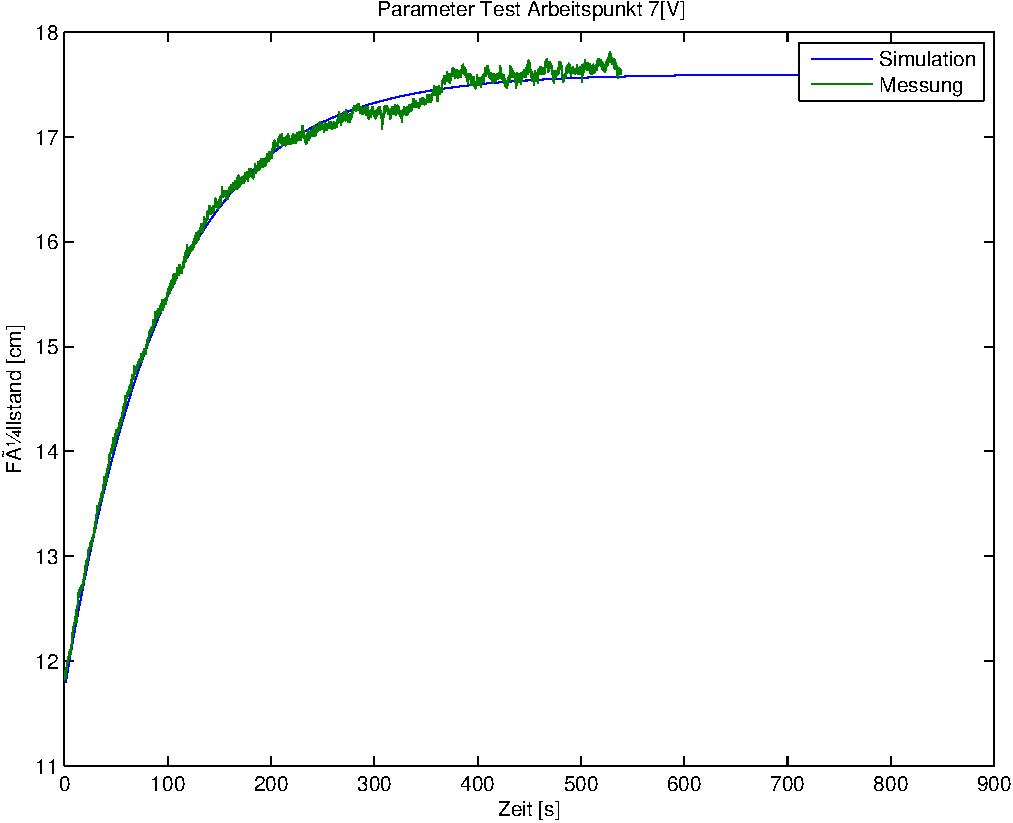
\includegraphics[width=1\textwidth]{07/parameter_test_7.pdf}
		\caption{Sprungantwort 7V zu 8V}
	\end{subfigure}
	\caption{Sprungantwortenvergleich von System und Modell}
\end{figure}
